\begin{figure}[!htb] 
	%\shorthandoff{;}
	\centering
	\resizebox{\textwidth}{!}{%
		\begin{minipage}[b]{.75\linewidth}
			\centering
			%\subfloat[\label{fig_exp_stability_map_a}]{
			\subcaptionbox{\label{subfig_exp_stability_map_a}}
			{
				\tikzsetnextfilename{fig_stability_map_a}
				\begin{tikzpicture}
					% color blind valid colors
					\definecolor{blueishGreen}{RGB}{0,158,15}
					\definecolor{skyBlue}{RGB}{86,180,233}
					\definecolor{orange}{RGB}{230,159,0}
					\definecolor{vermillon}{RGB}{213,94,0}
					\begin{axis}[
						name=stab_eg,
						width=.9\linewidth,
						%height=.7\columnwidth,
						ticklabel style = {font=\footnotesize},
						xlabel = $K_p$,
						%xlabel style = {yshift=1.15em, xshift=1.1em},
						ylabel = $K_i$,
						%ylabel style = {yshift=-1.5em},
						xmax = 2.2e-2,
						xmin = 0,
						ymax = 0.3,
						ymin = 0,
						%x tick scale label style={yshift=0.8em, xshift=0.5em},
						legend style={nodes={scale=0.75, transform shape}},
						]
						\draw[draw=white,line width=1pt,preaction={clip, postaction={pattern=north west lines, pattern color=blueishGreen}}] 
						(rel axis cs:0.0,0.0) -- (rel axis cs:0.0,0.63) -- (rel axis cs:0.67,0.67) -- (rel axis cs:0.67,0.55) -- (rel axis cs:0.75,0.32) -- (rel axis cs:0.88,0.23) -- (rel axis cs:0.92,0.0) -- cycle;
						\addplot[
							only marks, 
							vermillon,
							mark=square*, 
							mark size =1.1mm,
							mark options={fill opacity=0.75},
						] 
						table [y=ki, x=kp, col sep=comma]
						{misc/stability_mapping_stiff_unstable.csv};
						\label{plot:i}
						\addplot[
							only marks, 
							mark size =1.2mm,
							mark options={fill opacity=0.75},
							blueishGreen, 
						] 
						table [y=ki, x=kp, col sep=comma]
						{misc/stability_mapping_stiff_stable.csv};
						\label{plot:iv}
						\addplot[
							only marks,
							orange, 
							mark=pentagon*, 
							mark options={fill opacity=0.75},
							mark size = 1.3mm,
						] 
						table [y=ki, x=kp, col sep=comma]
						{misc/stability_mapping_stiff_critic.csv};
						\label{plot:ii}
						\addplot[
							only marks,
							skyBlue, 
							mark=triangle*, 
							mark options={fill opacity=0.75},
							mark size = 1.4mm,
						] 
						table [y=ki, x=kp, col sep=comma]
						{misc/stability_mapping_stiff_uncomf.csv};
						\label{plot:iii}
						\addplot [
							only marks,
							color=black,
							mark=star,
							mark size = 1.2mm,
						]
						table[row sep=crcr]{0.015	0.08\\} ;
						%\addlegendimage{/pgfplots/refstyle=plot:i}  \addlegendentry{(i)}
				        %\addlegendimage{/pgfplots/refstyle=plot:ii}  \addlegendentry{(ii)}
				        %\addlegendimage{/pgfplots/refstyle=plot:iii}  \addlegendentry{(iii)}
				        %\addlegendimage{/pgfplots/refstyle=plot:iv}  \addlegendentry{(iv)}
					\end{axis}
					\matrix [
			             matrix of nodes,
			             nodes={anchor=west},
			             anchor=north east,
			             at={([shift={(-3pt,-3pt)}]stab_eg.north east)},
			             fill=white,
			             draw,
			             inner sep=2pt,
			             row sep=1pt,
			             scale=0.75,
			            ] {
		           \ref{plot:i} \footnotesize{(i)}
		           \ref{plot:iii} \footnotesize{(iii)} \\
		           \ref{plot:ii} \footnotesize{(ii)} 
		           \ref{plot:iv} \footnotesize{(iv)} \\
		           };
				\end{tikzpicture}
			}
		\end{minipage}
		%
		\begin{minipage}[b]{.25\linewidth}
			\subcaptionbox{\label{subfig_exp_stability_map_b}}
			{
			%\subfloat[\label{fig_exp_stability_map_b}]{
				\centering
				\newcommand\funcA{1}
				\newcommand\funcW{2*pi}
				\newcommand\funcPhi{1/pi}
				\tikzsetnextfilename{fig_stability_map_b}
				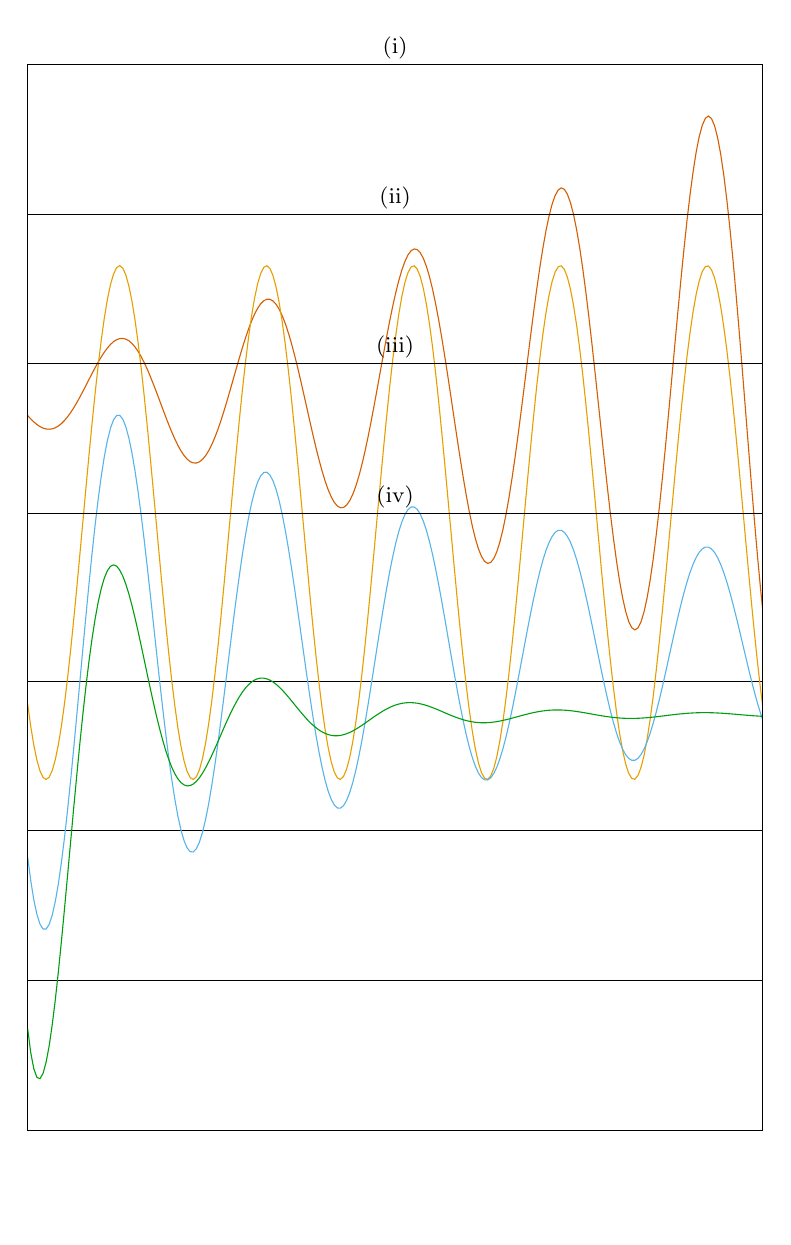
\begin{tikzpicture}[trim axis left, trim axis right]
					\definecolor{blueishGreen}{RGB}{0,158,15}
					\definecolor{skyBlue}{RGB}{86,180,233}
					\definecolor{orange}{RGB}{230,159,0}
					\definecolor{vermillon}{RGB}{213,94,0}
					\begin{scope}[yshift = 6.8cm]
						\begin{axis}[
							width=.9\linewidth,
							xmin=1,
							xmax=3,
							title={(i)},
							title style={font=\footnotesize, yshift=-0.75em},
							xtick=\empty,
							ytick=\empty]
							%
							\addplot[color=vermillon, variable=\t, domain=1:6, samples=600] {t^2*sin(deg(2*pi*2.5*t+pi/4))};
							%
						\end{axis}
					\end{scope}
					\begin{scope}[yshift = 4.9cm]
						\begin{axis}[
							width=.9\linewidth,
							xmin=1,
							xmax=3,
							title={(ii)},
							title style={font=\footnotesize, yshift=-0.75em},
							xtick=\empty,
							ytick=\empty]
							%
							\addplot[color=orange, variable=\t, domain=1:6, samples=600] {sin(deg(2*pi*2.5*t+pi/4))};
							%
						\end{axis}
					\end{scope}
					\begin{scope}[yshift = 3cm]
						\begin{axis}[
							width=.9\linewidth,
							xmin=1,
							xmax=3,
							title={(iii)},
							title style={font=\footnotesize, yshift=-0.75em},
							xtick=\empty,
							ytick=\empty]
							%
							\addplot[color=skyBlue, variable=\t, domain=1:6, samples=600] {1/t*sin(deg(2*pi*2.5*t+pi/4))};
							%
						\end{axis}
					\end{scope}
					\begin{scope}[yshift = 1.1cm]
						\begin{axis}[
							width=.9\linewidth,
							xmin=1,
							xmax=3,
							title={(iv)},
							title style={font=\footnotesize, yshift=-0.75em},
							xtick=\empty,
							ytick=\empty]
							%
							\addplot[color=blueishGreen, variable=\t, domain=1:6, samples=600] {(1/(t^5))*sin(deg(2*pi*2.5*t+pi/4))};
							%
						\end{axis}
					\end{scope}
					\draw[white] (0,0) -- (1,0);
				\end{tikzpicture}
			}
		\end{minipage}
	}
	%\shorthandon{;} 
	\caption{(\subref{subfig_exp_stability_map_a}) Cartographie expérimentale de la stabilité en fonction des gains du correcteur en admittance. Première condition : co-manipulation avec des co-contractions intentionnelles du bras et de la main (formes). Deuxième condition : co-manipulation avec des co-contractions nominales pour la tâche de jonglerie (la zone verte hachurée représente la catégorie (iv)). Les gains utilisés sur le banc expérimental sont indiqués par une étoile. (\subref{subfig_exp_stability_map_b}) Catégories typiques des réponses en force.}
	\label{fig_exp_stability_map}
\end{figure}